\documentclass[doubleside, titlepage]{article}
\usepackage{xcolor,listings}
\usepackage[utf8]{inputenc}
\usepackage[english]{babel}
\usepackage{textcomp}
\usepackage{graphicx}
\usepackage[papersize={210mm,297mm},top=2cm, bottom=2.25cm, left=1.8cm , right=1.8cm]{geometry}
\lstset{upquote=true}
\usepackage{amsmath}
\usepackage{tikz}
\usepackage{epigraph}
\usepackage{hyperref}
\hypersetup{
    linktoc=all
}
\usepackage{titlesec}
\usepackage{fancyhdr}
\pagestyle{fancy}
\usepackage{lastpage}

\renewcommand\headrulewidth{0.66pt}
\fancyhead[L]{\leftmark}
\fancyhead[R]{Spring 2016}

\renewcommand\footrulewidth{0.66pt}
\fancyfoot[L]{ ~\\ Group 3}
\fancyfoot[C]{ ~\\CS323 - Project delivrable \\ \textbf{Page \thepage/\pageref{LastPage}}}
\fancyfoot[R]{ ~\\ 
\includegraphics[scale=0.35]{epfl_logo}}

\fancypagestyle{firstpage}{%
    \fancyhf{}%
    \renewcommand\footrulewidth{0.66pt}
    \fancyfoot[L]{ ~\\ Group 3}
    \fancyfoot[C]{ ~\\CS323 - Project delivrable \\ \textbf{Page \thepage/\pageref{LastPage}}}
    \fancyfoot[R]{ ~\\ 
\includegraphics[scale=0.35]{epfl_logo}}
    \renewcommand{\headrulewidth}{0mm}%
}

\renewcommand\epigraphflush{center}
\renewcommand\epigraphsize{\normalsize}
\setlength\epigraphwidth{0.5\textwidth}
\setlength\epigraphrule{0.5pt}

\renewcommand{\textflush}{flushright} \renewcommand{\sourceflush}{flushright}

\let\originalepigraph\epigraph
\renewcommand\epigraph[2]{\originalepigraph{#1}{\textsc{#2}}}

\definecolor{titlepagecolor}{cmyk}{0,.9,0.7,0}

\DeclareFixedFont{\titlefont}{T1}{ppl}{b}{}{0.5in}

\makeatletter
\def\printauthor{%
    {\large \@author}}
\makeatother
\author{%
	~\\	~\\
    Jeremy Hottinger \\
    259573 \\
    \href{mailto:jeremy.hottinger@epfl.ch}{\texttt{jeremy.hottinger@epfl.ch}}\vspace{20pt} \\
    Aurélien Soccard \\
    235746 \\
    \href{mailto:aurelien.soccard@epfl.ch}{\texttt{aurelien.soccard@epfl.ch}}\vspace{20pt} \\
    Téo Stocco \\
    235744 \\
    \href{mailto:teo.stocco@epfl.ch}{\texttt{teo.stocco@epfl.ch}}\vspace{20pt} \\
    }

% The following code is borrowed from: http://tex.stackexchange.com/a/86310/10898

\newcommand\titlepagedecoration{%
\begin{tikzpicture}[remember picture,overlay,shorten >= -10pt]

\coordinate (aux1) at ([yshift=-15pt]current page.north east);
\coordinate (aux2) at ([yshift=-410pt]current page.north east);
\coordinate (aux3) at ([xshift=-4.5cm]current page.north east);
\coordinate (aux4) at ([yshift=-150pt]current page.north east);

\begin{scope}[titlepagecolor!40,line width=12pt,rounded corners=12pt]
\draw
  (aux1) -- coordinate (a)
  ++(225:5) --
  ++(-45:5.1) coordinate (b);
\draw[shorten <= -10pt]
  (aux3) --
  (a) --
  (aux1);
\draw[opacity=0.6,titlepagecolor,shorten <= -10pt]
  (b) --
  ++(225:2.2) --
  ++(-45:2.2);
\end{scope}
\draw[titlepagecolor,line width=8pt,rounded corners=8pt,shorten <= -10pt]
  (aux4) --
  ++(225:0.8) --
  ++(-45:0.8);
\begin{scope}[titlepagecolor!70,line width=6pt,rounded corners=8pt]
\draw[shorten <= -10pt]
  (aux2) --
  ++(225:3) coordinate[pos=0.45] (c) --
  ++(-45:3.1);
\draw
  (aux2) --
  (c) --
  ++(135:2.5) --
  ++(45:2.5) --
  ++(-45:2.5) coordinate[pos=0.3] (d);
\draw
  (d) -- +(45:1);
\end{scope}
\end{tikzpicture}%
}

\begin{document}
\begin{titlepage}
\thispagestyle{firstpage}
\vspace*{3cm}
\titlefont CS-323 : Project delivrable\par
\vspace*{0.5cm}
\epigraph{This is our first deliverable for the \textit{Bookshelf} project of the introduction to database course (spring 2016 - Pr. Anastasia Ailamaki), which sums up our ER-model and schema. It also contains some justifications.}%
{\textit{March 2016} - \textsc{Team n°3}}
\null\vfill
\vspace*{5cm}
\noindent
\hfill
\begin{minipage}{0.5\linewidth}
    \begin{flushright}
        \printauthor
    \end{flushright}
\end{minipage}
%
\begin{minipage}{0.02\linewidth}
    \rule{1pt}{175pt}
\end{minipage}
\titlepagedecoration
\end{titlepage}

\setcounter{tocdepth}{1}
\vspace{-1cm}
\tableofcontents

\newpage

\part{Delivrable 1}

\section{Justifications}

We started to take a look at the given data and tried to understand how tables where connected at a first glance by drawing a really simplified diagram. Once this was done, we started to look at more deeply to the data : how are they stored? May they be empty? Are they all relevant? Our major decision was not to drop any table, but only add and remove some fields to entities.
~\\~\\
First, for everything that is related to publications, we quickly figured out how things were working. Therefore, we quickly decided to drop some of the unused id (such as its publication author or its publication content). As a primary key, we made the choice to inflate it using constraints. Furthermore, we also decided to separate the price into two fields, one for the amount and one for the currency, this solution being much more efficient while looking for some price range for instance.
~\\~\\
Even though both publications and titles have each one a related type field we did not find it relevant to split them into different tables and/or explicit a IS-A relationship because of the way the datas are gathered.
~\\~\\
Another part of the work was to analyse how tables were connected to remove potential redundancy. For instance, an award has a category but also a type, and a category has a type. These two types being always the same, we needed to drop out some content, what we've done by removing the type entry in a award. We also realise that, for instance in the author table, among the 80'000 birth places, only 10\% were unique so we have started thinking about changing this attribute into a placeID and create a places table. There were some advantages (no redundancy, less space consumed) but some drawbacks (2 queries instead of one for each author) that finally made us stay with the given configuration (however, if another would be using a place, we will have done that).
~\\~\\
Furthermore, to write properly the creation of the table, we needed to know exactly what entry may be null, and which ones could not. This was done by inspecting carefully the data and reading correctly the instructions. Then, the dilemma was for notes and web pages tables. Indeed, for note, we only have two entries : the ID and the raw note, whereas for a website, there are an ID, an URL but also some other IDs to relate it to other entities : among these 7 IDs, only one   The type of each entry is explained in the following paragraph. Our final has been not the change the structure of these two tables since there is no WebpageID entry in tables as there is for note, but whether a web page is directly connected to the ID of its corresponding entity. Therefore, it implies to add an entry into these 7 tables, and we decided not to do this for practical reasons. Besides, we also thought about simply adding a simply URL entry into the note table, but this solution was also not satisfactory since before insert we would need to do a map from web page to note (not that hard) but since primary keys are only unique in one table, an author and a publication may have the same ID and this would imply much more work to know which website belongs to who.
~\\~\\
As publications and titles both have a type we used an enum as a compromise between having a raw string field and creating normalisation for it. This avoids the redundancy and increase data consistency. Note that it would not be an option if the dataset usage would include adding new types (normalising is better in this case).
~\\~\\
Last but not least, some intensive parsing has also been performed to know exactly how many characters were required for instance for each field, since we have encountered some difficulties with Cyrillic. We quickly realised that we should definitely parse these values before inserting them, it presents the advantages of being less memory consuming (6 characters become 1) and also the process of conversion is only done one time.
\addtocounter{page}{1}

\section{ER model}

This entity-relation model only contains fields which are either directly use for relation or as primary key (underline then). For a more complete view of the table, refers to the next section. Fields are coloured in blue, direct relationships in yellow, relationships through a table in red.
~\\
\textbf{Note :} If you find this diagram too small, a larger version is available online at the following address :
$$
\text{\href{https://documents.epfl.ch/users/s/so/soccard/private/DBMS}{\texttt{https://documents.epfl.ch/users/s/so/soccard/private/DBMS}}}
$$
\begin{flushright}
(access restricted to the db2016 group as defined in the EPFL AD directory).
\end{flushright}

\newpage

\begin{center}
    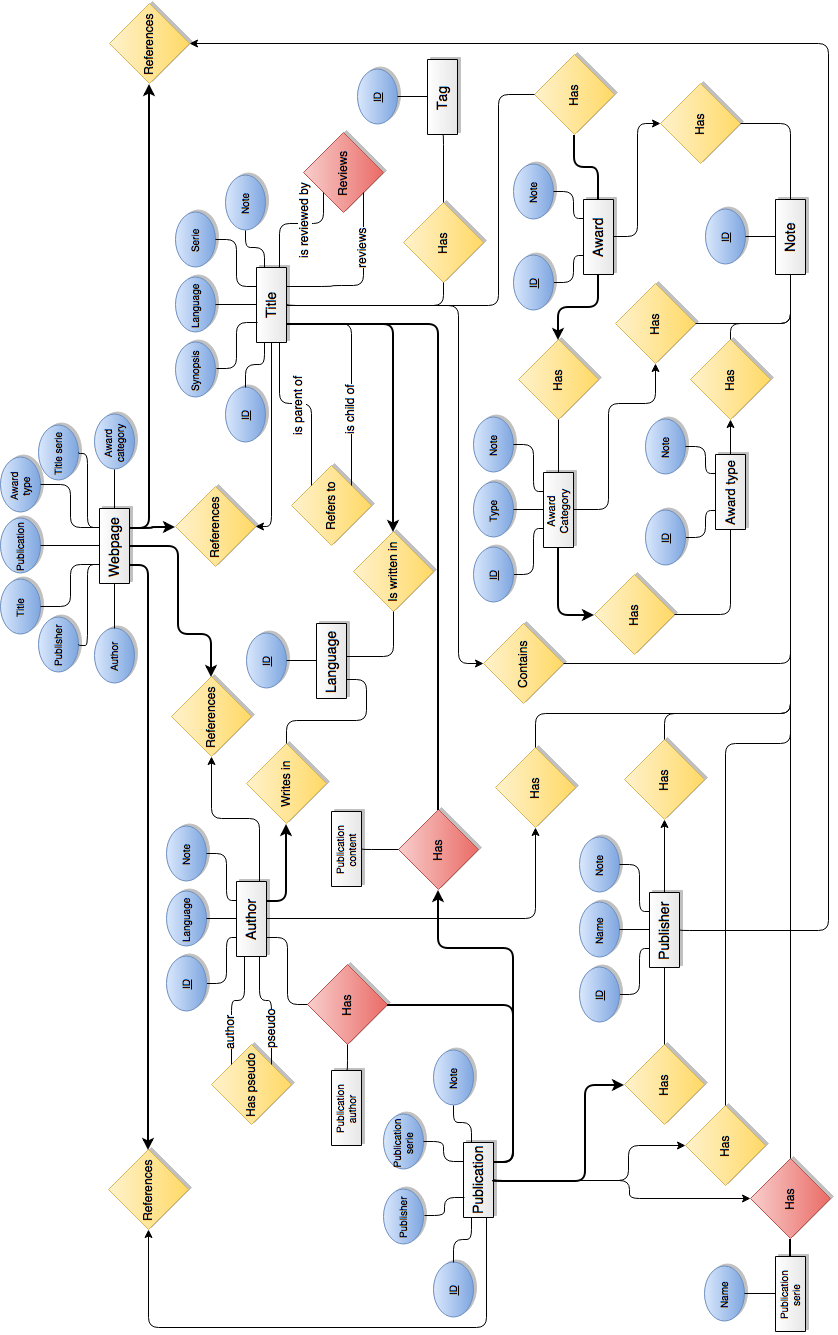
\includegraphics[scale = 0.5]{DBMS_ER}
\end{center}

\section{SQL schema}

\subsection{Entities}

\begin{lstlisting}[language=SQL,showspaces=false,basicstyle=\ttfamily,numberstyle=\tiny,commentstyle=\color{gray}
        ]
CREATE TYPE PUBLICATION_TYPE AS ENUM ('ANTHOLOGY', 'COLLECTION', 'MAGAZINE',
	'NONFICTION', 'NOVEL', 'OMNIBUS', 'FANZINE', 'CHAPBOOK');
\end{lstlisting}

\begin{lstlisting}[language=SQL,showspaces=false,basicstyle=\ttfamily,numberstyle=\tiny,commentstyle=\color{gray}
        ]
CREATE TYPE TITLE_TYPE AS ENUM ('ANTHOLOGY', 'BACKCOVERART', 'COLLECTION',
	'COVERART', 'INTERIORART', 'EDITOR', 'ESSAY', 'INTERVIEW', 'NOVEL',
	'NONFICTION', 'OMNIBUS', 'POEM', 'REVIEW', 'SERIAL', 'SHORTFICTION',
	'CHAPBOOK');
\end{lstlisting}

\begin{lstlisting}[language=SQL,showspaces=false,basicstyle=\ttfamily,numberstyle=\tiny,commentstyle=\color{gray}
        ]
CREATE TABLE authors
(
  id          INT PRIMARY KEY NOT NULL,
  name        VARCHAR(256)    NOT NULL,
  legal_name  VARCHAR(256),
  last_name   VARCHAR(256),
  pseudonym   INT, -- fk
  birth_place VARCHAR(256),
  birth_date  DATE,
  death_date  DATE,
  email       VARCHAR(256),
  image       VARCHAR(256),
  language_id INT, -- fk
  note_id     INT -- fk
)
\end{lstlisting}

\begin{lstlisting}[language=SQL,showspaces=false,basicstyle=\ttfamily,numberstyle=\tiny,commentstyle=\color{gray}
        ]
CREATE TABLE publications
(
  id             INT PRIMARY KEY 	NOT NULL,
  title          VARCHAR(256)    	NOT NULL,
  date_pub       DATE            	NOT NULL,
  publisher_id   INT             	NOT NULL, -- fk
  pages          INT,
  preface        INT,
  packaging_type VARCHAR(16)   		NOT NULL,
  type           PUBLICATON_TYPE    NOT NULL,
  isbn           BIGINT,
  cover          VARCHAR(256),
  price          FLOAT,
  currency       VARCHAR(8),
  pub_series_id  INT, -- fk
  pub_series_num INT,
  note_id        INT -- fk
)
\end{lstlisting}

\newpage

\begin{lstlisting}[language=SQL,showspaces=false,basicstyle=\ttfamily,numberstyle=\tiny,commentstyle=\color{gray}
        ]
CREATE TABLE titles
(
  id           INT PRIMARY KEY NOT NULL,
  title        VARCHAR(256)    NOT NULL,
  translator   VARCHAR(256),
  synopsis     INT, -- fk
  note_id      INT, -- fk
  series_id    INT, -- fk
  series_num   INT,
  story_length VARCHAR(256),
  type         TITLE_TYPE,
  parent       INT             NOT NULL DEFAULT 0, -- fk
  language_id  INT, -- fk
  graphic      BOOLEAN         NOT NULL
)
\end{lstlisting}

\begin{lstlisting}[language=SQL,showspaces=false,basicstyle=\ttfamily,numberstyle=\tiny,commentstyle=\color{gray}
        ]
CREATE TABLE languages
(
  id     INT PRIMARY KEY NOT NULL,
  name   VARCHAR(256)    NOT NULL,
  code   CHAR(3)         NOT NULL UNIQUE,
  script BOOLEAN
)
\end{lstlisting}

\begin{lstlisting}[language=SQL,showspaces=false,basicstyle=\ttfamily,numberstyle=\tiny,commentstyle=\color{gray}
        ]
CREATE TABLE notes
(
  id   INT PRIMARY KEY NOT NULL,
  note TEXT            NOT NULL
)
\end{lstlisting}

\begin{lstlisting}[language=SQL,showspaces=false,basicstyle=\ttfamily,numberstyle=\tiny,commentstyle=\color{gray}
        ]
CREATE TABLE webpages
(
  id                     INT PRIMARY KEY NOT NULL,
  author_id              INT, -- fk
  publisher_id           INT, -- fk
  title_id               INT, -- fk
  url                    VARCHAR(256)    NOT NULL UNIQUE,
  publications_series_id INT, -- fk
  award_type_id          INT, -- fk
  title_series_id        INT, -- fk
  award_category_id      INT -- fk
)
\end{lstlisting}

\begin{lstlisting}[language=SQL,showspaces=false,basicstyle=\ttfamily,numberstyle=\tiny,commentstyle=\color{gray}
        ]
CREATE TABLE tags
(
  id   INT PRIMARY KEY NOT NULL,
  name VARCHAR(256)    NOT NULL
)
\end{lstlisting}

\begin{lstlisting}[language=SQL,showspaces=false,basicstyle=\ttfamily,numberstyle=\tiny,commentstyle=\color{gray}
        ]
CREATE TABLE titles_series
(
  id      INT PRIMARY KEY NOT NULL,
  title   VARCHAR(256)    NOT NULL,
  parent  INT DEFAULT 0, -- fk
  note_id INT -- fk
)
\end{lstlisting}

\newpage

\begin{lstlisting}[language=SQL,showspaces=false,basicstyle=\ttfamily,numberstyle=\tiny,commentstyle=\color{gray}
        ]
CREATE TABLE awards
(
  id          INT PRIMARY KEY NOT NULL,
  title       VARCHAR(256)    NOT NULL,
  date        DATE            NOT NULL,
  category_id INT             NOT NULL, -- fk
  note_id     INT -- fk
)
\end{lstlisting}

\begin{lstlisting}[language=SQL,showspaces=false,basicstyle=\ttfamily,numberstyle=\tiny,commentstyle=\color{gray}
        ]
CREATE TABLE awards_categories
(
  id      INT PRIMARY KEY NOT NULL,
  name    VARCHAR(256)    NOT NULL,
  type_id INT             NOT NULL, -- fk
  ordr    INT,
  note_id INT -- fk
)
\end{lstlisting}

\begin{lstlisting}[language=SQL,showspaces=false,basicstyle=\ttfamily,numberstyle=\tiny,commentstyle=\color{gray}
        ]
CREATE TABLE awards_types
(
  id          INT PRIMARY KEY NOT NULL,
  code        CHAR(2) UNIQUE,
  name        VARCHAR(256)    NOT NULL,
  note_id     INT, -- fk
  awarded_by  VARCHAR(256)    NOT NULL,
  awarded_for VARCHAR(256)    NOT NULL,
  short_name  VARCHAR(256)    NOT NULL UNIQUE,
  poll        BOOLEAN         NOT NULL,
  non_genre   BOOLEAN         NOT NULL
)
\end{lstlisting}

\begin{lstlisting}[language=SQL,showspaces=false,basicstyle=\ttfamily,numberstyle=\tiny,commentstyle=\color{gray}
        ]
CREATE TABLE publishers
(
  id      INT PRIMARY KEY NOT NULL,
  name    VARCHAR(512)    NOT NULL,
  note_id INT -- fk
)
\end{lstlisting}

\begin{lstlisting}[language=SQL,showspaces=false,basicstyle=\ttfamily,numberstyle=\tiny,commentstyle=\color{gray}
        ]
CREATE TABLE publications_series
(
  id      INT PRIMARY KEY NOT NULL,
  name    VARCHAR(512)    NOT NULL,
  note_id INT -- fk
)
\end{lstlisting}

\subsection{Relations}

\begin{lstlisting}[language=SQL,showspaces=false,basicstyle=\ttfamily,numberstyle=\tiny,commentstyle=\color{gray}
        ]
CREATE TABLE publications_authors
(
  publication_id INT NOT NULL, -- fk
  author_id      INT NOT NULL, -- fk
  CONSTRAINT pk_publications_authors PRIMARY KEY (publication_id, author_id)
)
\end{lstlisting}

\begin{lstlisting}[language=SQL,showspaces=false,basicstyle=\ttfamily,numberstyle=\tiny,commentstyle=\color{gray}
        ]
CREATE TABLE titles_awards
(
  title_id INT NOT NULL, -- fk
  award_id INT NOT NULL, -- fk
  CONSTRAINT pk_titles_awards PRIMARY KEY (title_id, award_id)
)
\end{lstlisting}

\begin{lstlisting}[language=SQL,showspaces=false,basicstyle=\ttfamily,numberstyle=\tiny,commentstyle=\color{gray}
        ]
CREATE TABLE titles_tags
(
  title_id INT NOT NULL, -- fk
  tag_id   INT NOT NULL, -- fk
  CONSTRAINT pk_titles_tags PRIMARY KEY (title_id, tag_id)
)
\end{lstlisting}

\begin{lstlisting}[language=SQL,showspaces=false,basicstyle=\ttfamily,numberstyle=\tiny,commentstyle=\color{gray}
        ]
CREATE TABLE reviews
(
  title_id  INT NOT NULL, -- fk
  review_id INT NOT NULL, -- fk
  CONSTRAINT pk_reviews PRIMARY KEY (title_id, review_id)
)
\end{lstlisting}

\begin{lstlisting}[language=SQL,showspaces=false,basicstyle=\ttfamily,numberstyle=\tiny,commentstyle=\color{gray}
        ]
CREATE TABLE publications_contents
(
  title_id       INT NOT NULL, -- fk
  publication_id INT NOT NULL, -- fk
  CONSTRAINT pk_publications_contents PRIMARY KEY (title_id, publication_id)
)
\end{lstlisting}


\subsection{Foreign keys}

\subsubsection{Authors}
\begin{tabular}{ ll }
\begin{minipage}{3in}
\begin{lstlisting}[language=SQL,showspaces=false,basicstyle=\ttfamily,numberstyle=\tiny,commentstyle=\color{gray}
        ]
ALTER TABLE authors
ADD FOREIGN KEY (language_id)
REFERENCES languages (id)
ON DELETE SET NULL;
\end{lstlisting}
\end{minipage}
&
\begin{minipage}{3in}
\begin{lstlisting}[language=SQL,showspaces=false,basicstyle=\ttfamily,numberstyle=\tiny,commentstyle=\color{gray}
        ]
ALTER TABLE authors
ADD FOREIGN KEY (pseudonym)
REFERENCES authors (id)
ON DELETE CASCADE;
\end{lstlisting}
\end{minipage}
\\
\begin{minipage}{3in}
\begin{lstlisting}[language=SQL,showspaces=false,basicstyle=\ttfamily,numberstyle=\tiny,commentstyle=\color{gray}
        ]
ALTER TABLE authors
ADD FOREIGN KEY (note_id)
REFERENCES notes (id)
ON DELETE SET NULL;
\end{lstlisting}

\end{minipage}
\end{tabular}

\subsubsection{Publication authors}
\begin{tabular}{ ll }
\begin{minipage}{3in}
\begin{lstlisting}[language=SQL,showspaces=false,basicstyle=\ttfamily,numberstyle=\tiny,commentstyle=\color{gray}
        ]
ALTER TABLE publications_authors
ADD FOREIGN KEY (publication_id)
REFERENCES publications (id)
ON DELETE CASCADE;
\end{lstlisting}
\end{minipage}
&
\begin{minipage}{3in}
\begin{lstlisting}[language=SQL,showspaces=false,basicstyle=\ttfamily,numberstyle=\tiny,commentstyle=\color{gray}
        ]
ALTER TABLE publications_authors
ADD FOREIGN KEY (author_id)
REFERENCES authors (id)
ON DELETE CASCADE;
\end{lstlisting}
\end{minipage}
\end{tabular}

\subsubsection{Publications}
\begin{tabular}{ ll }
\begin{minipage}{3in}
\begin{lstlisting}[language=SQL,showspaces=false,basicstyle=\ttfamily,numberstyle=\tiny,commentstyle=\color{gray}
        ]
ALTER TABLE publications
ADD FOREIGN KEY (publisher_id)
REFERENCES publishers (id)
ON DELETE SET NULL;
\end{lstlisting}
\end{minipage}
&
\begin{minipage}{3in}
\begin{lstlisting}[language=SQL,showspaces=false,basicstyle=\ttfamily,numberstyle=\tiny,commentstyle=\color{gray}
        ]
ALTER TABLE publications
ADD FOREIGN KEY (pub_series_id)
REFERENCES publications_series (id)
ON DELETE SET NULL;
\end{lstlisting}
\end{minipage}
\\
\begin{minipage}{3in}
\begin{lstlisting}[language=SQL,showspaces=false,basicstyle=\ttfamily,numberstyle=\tiny,commentstyle=\color{gray}
        ]
ALTER TABLE publications
ADD FOREIGN KEY (note_id)
REFERENCES notes (id)
ON DELETE SET NULL;
\end{lstlisting}
\end{minipage}
\end{tabular}

\subsubsection{Publication contents}
\begin{tabular}{ ll }
\begin{minipage}{3in}
\begin{lstlisting}[language=SQL,showspaces=false,basicstyle=\ttfamily,numberstyle=\tiny,commentstyle=\color{gray}
        ]
ALTER TABLE publications_contents
ADD FOREIGN KEY (title_id)
REFERENCES titles (id)
ON DELETE CASCADE;
\end{lstlisting}
\end{minipage}
&
\begin{minipage}{3in}
\begin{lstlisting}[language=SQL,showspaces=false,basicstyle=\ttfamily,numberstyle=\tiny,commentstyle=\color{gray}
        ]
ALTER TABLE publications_contents
ADD FOREIGN KEY (publication_id)
REFERENCES publications (id)
ON DELETE CASCADE;
\end{lstlisting}
\end{minipage}
\end{tabular}

\subsubsection{Publishers}
\begin{lstlisting}[language=SQL,showspaces=false,basicstyle=\ttfamily,numberstyle=\tiny,commentstyle=\color{gray}
        ]
ALTER TABLE publishers
ADD FOREIGN KEY (note_id)
REFERENCES notes (id)
ON DELETE SET NULL;
\end{lstlisting}

\subsubsection{Publication series}
\begin{lstlisting}[language=SQL,showspaces=false,basicstyle=\ttfamily,numberstyle=\tiny,commentstyle=\color{gray}
        ]
ALTER TABLE publications_series
ADD FOREIGN KEY (note_id)
REFERENCES notes (id)
ON DELETE SET NULL;
\end{lstlisting}

\subsubsection{Titles}
\begin{tabular}{ ll }
\begin{minipage}{3in}
\begin{lstlisting}[language=SQL,showspaces=false,basicstyle=\ttfamily,numberstyle=\tiny,commentstyle=\color{gray}
        ]
ALTER TABLE titles
ADD FOREIGN KEY (synopsis)
REFERENCES notes (id)
ON DELETE SET NULL;
\end{lstlisting}
\end{minipage}
&
\begin{minipage}{3in}
\begin{lstlisting}[language=SQL,showspaces=false,basicstyle=\ttfamily,numberstyle=\tiny,commentstyle=\color{gray}
        ]
ALTER TABLE titles
ADD FOREIGN KEY (series_id)
REFERENCES titles_series (id)
ON DELETE SET NULL;
\end{lstlisting}
\end{minipage}
\\
\begin{minipage}{3in}
\begin{lstlisting}[language=SQL,showspaces=false,basicstyle=\ttfamily,numberstyle=\tiny,commentstyle=\color{gray}
        ]
ALTER TABLE titles
ADD FOREIGN KEY (parent)
REFERENCES titles (id)
ON DELETE SET DEFAULT;
\end{lstlisting}
\end{minipage}
&
\begin{minipage}{3in}
\begin{lstlisting}[language=SQL,showspaces=false,basicstyle=\ttfamily,numberstyle=\tiny,commentstyle=\color{gray}
        ]
ALTER TABLE titles
ADD FOREIGN KEY (language_id)
REFERENCES languages (id)
ON DELETE SET NULL;
\end{lstlisting}
\end{minipage}
\\
\begin{minipage}{3in}
\begin{lstlisting}[language=SQL,showspaces=false,basicstyle=\ttfamily,numberstyle=\tiny,commentstyle=\color{gray}
        ]
ALTER TABLE titles
ADD FOREIGN KEY (note_id)
REFERENCES notes (id)
ON DELETE SET NULL;
\end{lstlisting}
\end{minipage}
\end{tabular}

\subsubsection{Reviews}
\begin{tabular}{ ll }
\begin{minipage}{3in}
\begin{lstlisting}[language=SQL,showspaces=false,basicstyle=\ttfamily,numberstyle=\tiny,commentstyle=\color{gray}
        ]
ALTER TABLE reviews
ADD FOREIGN KEY (title_id)
REFERENCES titles (id)
ON DELETE CASCADE;
\end{lstlisting}
\end{minipage}
&
\begin{minipage}{3in}
\begin{lstlisting}[language=SQL,showspaces=false,basicstyle=\ttfamily,numberstyle=\tiny,commentstyle=\color{gray}
        ]
ALTER TABLE reviews
ADD FOREIGN KEY (review_id)
REFERENCES titles (id)
ON DELETE CASCADE;
\end{lstlisting}
\end{minipage}
\end{tabular}

\subsubsection{Webpages}
\begin{tabular}{ ll }
\begin{minipage}{3in}
\begin{lstlisting}[language=SQL,showspaces=false,basicstyle=\ttfamily,numberstyle=\tiny,commentstyle=\color{gray}
        ]
ALTER TABLE webpages
ADD FOREIGN KEY (author_id)
REFERENCES authors (id)
ON DELETE CASCADE;
\end{lstlisting}
\end{minipage}
 &
\begin{minipage}{3in}
\begin{lstlisting}[language=SQL,showspaces=false,basicstyle=\ttfamily,numberstyle=\tiny,commentstyle=\color{gray}
        ]
ALTER TABLE webpages
ADD FOREIGN KEY (publisher_id)
REFERENCES publishers (id)
ON DELETE CASCADE;
\end{lstlisting}
\end{minipage}
 \\
\begin{minipage}{3in}
\begin{lstlisting}[language=SQL,showspaces=false,basicstyle=\ttfamily,numberstyle=\tiny,commentstyle=\color{gray}
        ]
ALTER TABLE webpages
ADD FOREIGN KEY (title_id)
REFERENCES titles (id)
ON DELETE CASCADE;
\end{lstlisting}
\end{minipage}
 &
\begin{minipage}{3in}
\begin{lstlisting}[language=SQL,showspaces=false,basicstyle=\ttfamily,numberstyle=\tiny,commentstyle=\color{gray}
        ]
ALTER TABLE webpages
ADD FOREIGN KEY (publications_series_id)
REFERENCES publications_series (id)
ON DELETE CASCADE;
\end{lstlisting}
\end{minipage}
 \\
\begin{minipage}{3in}
\begin{lstlisting}[language=SQL,showspaces=false,basicstyle=\ttfamily,numberstyle=\tiny,commentstyle=\color{gray}
        ]
ALTER TABLE webpages
ADD FOREIGN KEY (award_type_id)
REFERENCES awards_types (id)
ON DELETE CASCADE;
\end{lstlisting}
\end{minipage}
 &
\begin{minipage}{3in}
\begin{lstlisting}[language=SQL,showspaces=false,basicstyle=\ttfamily,numberstyle=\tiny,commentstyle=\color{gray}
        ]
ALTER TABLE webpages
ADD FOREIGN KEY (title_series_id)
REFERENCES title_series (id)
ON DELETE CASCADE;
\end{lstlisting}
\end{minipage}
 \\
\begin{minipage}{3in}
\begin{lstlisting}[language=SQL,showspaces=false,basicstyle=\ttfamily,numberstyle=\tiny,commentstyle=\color{gray}
        ]
ALTER TABLE webpages
ADD FOREIGN KEY (award_category_id)
REFERENCES awards_categories (id)
ON DELETE CASCADE;
\end{lstlisting}
\end{minipage}
\end{tabular}

\subsubsection{Title awards}
\begin{tabular}{ ll }
\begin{minipage}{3in}
\begin{lstlisting}[language=SQL,showspaces=false,basicstyle=\ttfamily,numberstyle=\tiny,commentstyle=\color{gray}
        ]
ALTER TABLE titles_awards
ADD FOREIGN KEY (title_id)
REFERENCES titles (id)
ON DELETE CASCADE;
\end{lstlisting}
\end{minipage}
 &
\begin{minipage}{3in}
\begin{lstlisting}[language=SQL,showspaces=false,basicstyle=\ttfamily,numberstyle=\tiny,commentstyle=\color{gray}
        ]
ALTER TABLE titles_awards
ADD FOREIGN KEY (award_id)
REFERENCES awards (id)
ON DELETE CASCADE;
\end{lstlisting}
\end{minipage}
\end{tabular}

\subsubsection{Title tags}
\begin{tabular}{ ll }
\begin{minipage}{3in}
\begin{lstlisting}[language=SQL,showspaces=false,basicstyle=\ttfamily,numberstyle=\tiny,commentstyle=\color{gray}
        ]
ALTER TABLE titles_tags
ADD FOREIGN KEY (title_id)
REFERENCES titles (id)
ON DELETE CASCADE;
\end{lstlisting}
\end{minipage}
 &
\begin{minipage}{3in}
\begin{lstlisting}[language=SQL,showspaces=false,basicstyle=\ttfamily,numberstyle=\tiny,commentstyle=\color{gray}
        ]
ALTER TABLE titles_tags
ADD FOREIGN KEY (tag_id)
REFERENCES tags (id)
ON DELETE CASCADE;
\end{lstlisting}
\end{minipage}
 \\
\begin{minipage}{3in}
\begin{lstlisting}[language=SQL,showspaces=false,basicstyle=\ttfamily,numberstyle=\tiny,commentstyle=\color{gray}
        ]
ALTER TABLE title_series
ADD FOREIGN KEY (parent)
REFERENCES title_series (id)
ON DELETE SET DEFAULT;
\end{lstlisting}
\end{minipage}
 &
\begin{minipage}{3in}
\begin{lstlisting}[language=SQL,showspaces=false,basicstyle=\ttfamily,numberstyle=\tiny,commentstyle=\color{gray}
        ]
ALTER TABLE title_series
ADD FOREIGN KEY (note_id)
REFERENCES notes (id)
ON DELETE SET NULL;
\end{lstlisting}
\end{minipage}
\end{tabular}

\subsubsection{Awards}
\begin{tabular}{ ll }
\begin{minipage}{3in}
\begin{lstlisting}[language=SQL,showspaces=false,basicstyle=\ttfamily,numberstyle=\tiny,commentstyle=\color{gray}
        ]
ALTER TABLE awards
ADD FOREIGN KEY (category_id)
REFERENCES awards_categories (id)
ON DELETE SET NULL;
\end{lstlisting}
\end{minipage}
 &
\begin{minipage}{3in}
\begin{lstlisting}[language=SQL,showspaces=false,basicstyle=\ttfamily,numberstyle=\tiny,commentstyle=\color{gray}
        ]
ALTER TABLE awards
ADD FOREIGN KEY (note_id)
REFERENCES notes (id)
ON DELETE SET NULL;
\end{lstlisting}
\end{minipage}
\end{tabular}

\subsubsection{Award categories}

\begin{tabular}{ ll }
\begin{minipage}{3in}
\begin{lstlisting}[language=SQL,showspaces=false,basicstyle=\ttfamily,numberstyle=\tiny,commentstyle=\color{gray}
        ]
ALTER TABLE awards_categories
ADD FOREIGN KEY (type_id)
REFERENCES awards_types (id)
ON DELETE SET NULL;
\end{lstlisting}
\end{minipage}
 &
\begin{minipage}{3in}
\begin{lstlisting}[language=SQL,showspaces=false,basicstyle=\ttfamily,numberstyle=\tiny,commentstyle=\color{gray}
        ]
ALTER TABLE awards_categories
ADD FOREIGN KEY (note_id)
REFERENCES notes (id)
ON DELETE SET NULL;
\end{lstlisting}
\end{minipage}
\end{tabular}

\subsubsection{Award types}
\begin{lstlisting}[language=SQL,showspaces=false,basicstyle=\ttfamily,numberstyle=\tiny,commentstyle=\color{gray}
        ]
ALTER TABLE awards_types
ADD FOREIGN KEY (note_id)
REFERENCES notes (id)
ON DELETE SET NULL;
\end{lstlisting}

~\\
~\\
~\\

\section{Appendix : Relational Model}

\newpage

\begin{center}
    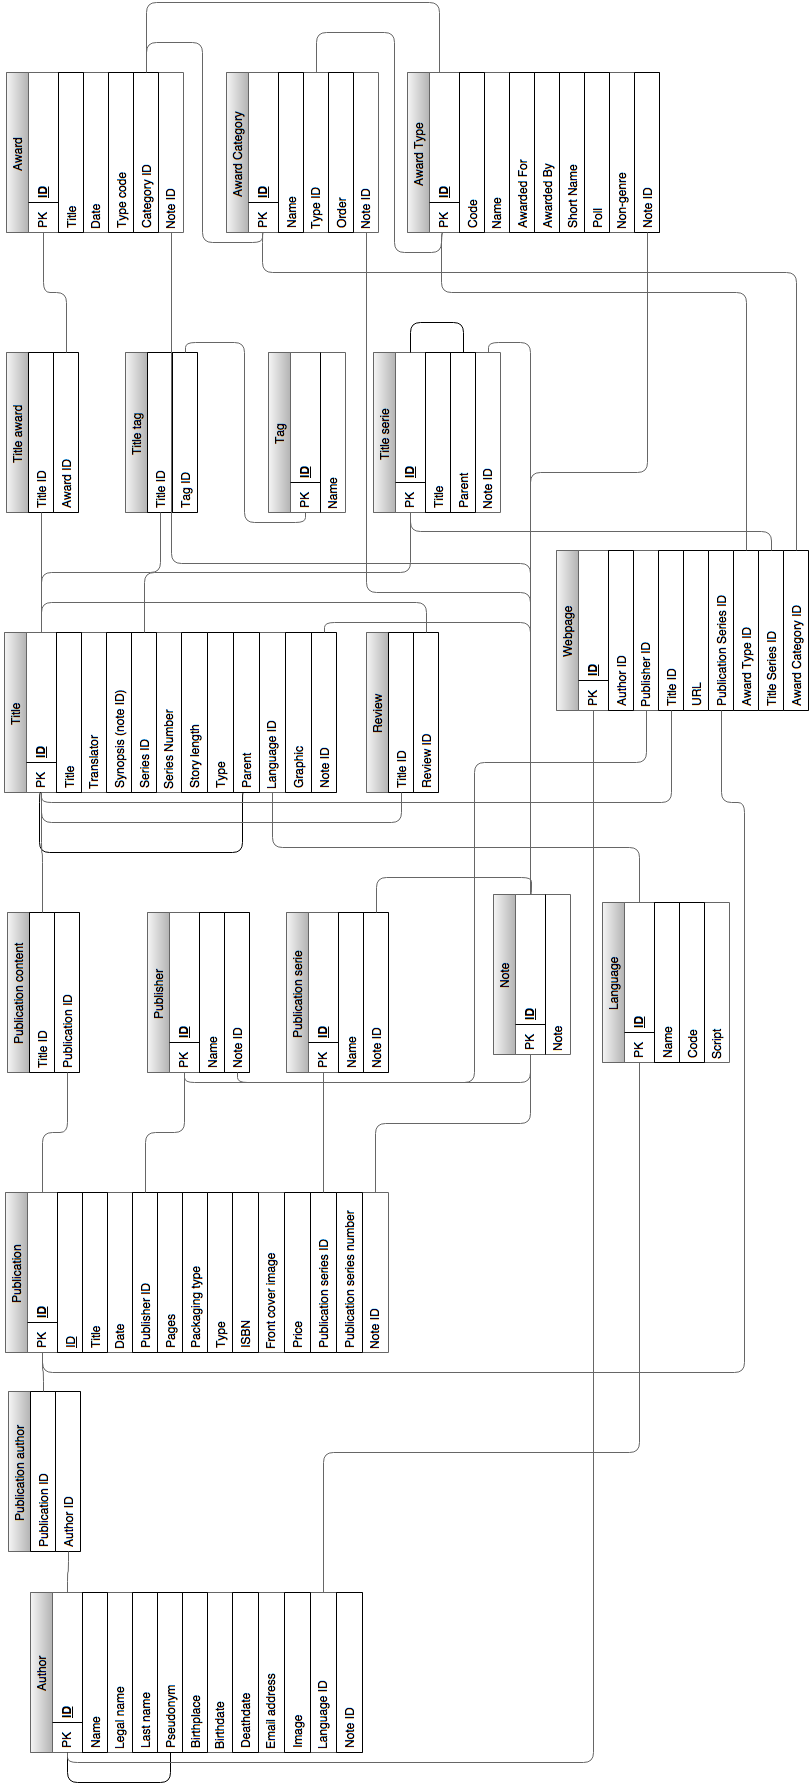
\includegraphics[scale = 0.4]{DBMS}
\end{center}

\part{Delivrable 2}
\section{Modifications of the previous milestone regarding remarks}

\subsection{Justifications}
We are now considering \texttt{Award\char`_Category} as a weak entity of \texttt{Award\char`_Type} since it doesn’t make sense for a category to exist without type. Therefore, the primary key of the category is now not only \texttt{cat\char`_ID} but also a tuple containing \texttt{cat\char`_ID} and \texttt{type\char`_ID}. This leads us to store again in our Award table the \texttt{type\char`_ID} attribute to make the connection between awards and their categories.

After analyzing the data, the graphic attribute may be null, we lead us to remove the NOT NULL constraint on this attribute.


\subsection{New ER Model}
\newpage
\section{Queries implementation}

\begin{enumerate}
\item For every year, output the year and the number of publications for said year.
	\begin{enumerate}
	\item Description of logic : We are using the \texttt{DATE\char`_PART} function provided by Postgresql to extract the year of the date stored for each publication. Then
      we simply do a GROUP BY on the year and count the number of entries.
	\item SQL statement :
		\begin{lstlisting}[language=SQL,showspaces=false,basicstyle=\ttfamily,numberstyle=\tiny,commentstyle=\color{gray}]
SELECT DATE_PART('year', p.date_pub) AS year, COUNT(*) AS count
FROM publications p
GROUP BY DATE_PART('year', p.date_pub)
ORDER BY year ASC;
		\end{lstlisting}

	\item Results (partial):\\

	\begin{tabular}{|l|c|r|}
  \hline
  year & count \\
  \hline
2005 & 	8667\\
2006 & 	8166\\
2007 & 	11970\\
2008 & 	14204\\
2009 & 	15526\\
2010 & 	19150\\
2011 & 	22470\\
2012 & 	22317\\
2013 & 	22923\\
2014 & 	21219\\
2015 & 	17206\\
2016 & 	1590\\
8888 & 	445\\
9999 & 	4\\
\hline
\end{tabular}

	\end{enumerate}
\item Output the names of the ten authors with most publications.

		\begin{enumerate}
	\item Description of logic : This query simply joins the authors and their publications and then GROUP BY on the author’s name. We just have to count the number of entries, ORDER BY that count and set a limit to 10.
	\item SQL statement :
		\begin{lstlisting}[language=SQL,showspaces=false,basicstyle=\ttfamily,numberstyle=\tiny,commentstyle=\color{gray}]
SELECT a.name, COUNT(*) AS count
FROM publications_authors p
INNER JOIN authors a ON p.author_id = a.id
GROUP BY a.name
ORDER BY count DESC
LIMIT 10;
		\end{lstlisting}

	\item Results :\\

	\begin{tabular}{|l|c|r|}
  \hline
  name & count \\
  \hline
uncredited & 2912\\
Isaac Asimov & 2389\\
Edgar Rice Burroughs & 2287\\
Robert A. Heinlein	& 1878\\
Arthur C. Clarke & 1512\\
Andre Norton & 1505\\
Stephen King & 1504\\
Robert Silverberg & 1481\\
Philip K. Dick & 1398\\
Terry Pratchett	& 1354\\
  \hline
\end{tabular}

	\end{enumerate}
\newpage
\item What are the names of the youngest and oldest authors to publish something in 2010?

			\begin{enumerate}
	\item Description of logic : Slightly more complicated this query uses nested subqueries to first select publications of 2010, then to select the maximum and minimum  birth dates of author that have some publication of 2010.
	\item SQL statement :
		\begin{lstlisting}[language=SQL,showspaces=false,basicstyle=\ttfamily,numberstyle=\tiny,commentstyle=\color{gray}]
SELECT a.name
FROM authors a
WHERE a.birth_date = (
SELECT MAX(a.birth_date) AS max
FROM publications_authors pa
JOIN authors a ON pa.author_id = a.id
WHERE pa.publication_id IN (
  SELECT pub.id
  FROM publications pub
  WHERE DATE_PART('year', pub.date_pub) = '2010'
)) OR
a.birth_date = (
SELECT MIN(a.birth_date) AS max
FROM publications_authors pa
JOIN authors A ON pa.author_id = a.id
WHERE pa.publication_id IN (
  SELECT pub.id
  FROM publications pub
  WHERE DATE_PART('year', pub.date_pub) = '2010'
));
		\end{lstlisting}

	\item Results :\\

	\begin{tabular}{|l|c|r|}
  \hline
  name \\
  \hline
Robert Henryson\\
Gavin Douglas\\
Greg Kurzawa\\
Laramie Sasseville\\
Brooke Vaughn\\
Pancham Yadav\\
Euripides\\
Aubrey Smith\\
Augustin Lardy\\
Livy\\
Michel Saint-Romain\\
Gan Bao\\
Timothy F. Mitchell\\
Gottfried von Strassburg\\
  \hline
\end{tabular}

	\end{enumerate}

\item How many comics (graphic titles) have publications with less than 50 pages, less than 100 pages, and more (or equal) than 100 pages?

	\begin{enumerate}
	\item Description of logic : After joining titles and publications, filtering them using the “graphic” field of titles and setting the condition on the number of pages, we just have to count the number of entries.
	\item SQL statement :
		\begin{lstlisting}[language=SQL,showspaces=false,basicstyle=\ttfamily,numberstyle=\tiny,commentstyle=\color{gray}]
SELECT COUNT(*)
FROM titles t
JOIN publications_contents AS pc ON t.id = pc.title_id
JOIN publications AS p ON pc.publication_id = p.id
WHERE t.graphic = 'YES'
AND p.Pages < 50;

------------------------------------------------

SELECT COUNT(*)
FROM titles t
JOIN publications_contents AS pc ON t.id = pc.title_id
JOIN publications AS p ON pc.publication_id = p.id
WHERE t.graphic = 'YES'
AND p.Pages < 100;

------------------------------------------------

SELECT COUNT(*)
FROM titles t
JOIN publications_contents AS pc ON t.id = pc.title_id
JOIN publications AS p ON pc.publication_id = p.id
WHERE t.graphic = 'YES'
AND p.Pages >= 100;
		\end{lstlisting}

	\item Results :\\

	\begin{tabular}{|l|c|r|}
	  \hline
		count \\
	  \hline
		153\\
	  \hline
	\end{tabular}

	\begin{tabular}{|l|c|r|}
	  \hline
		count \\
	  \hline
		202\\
	  \hline
	\end{tabular}

	\begin{tabular}{|l|c|r|}
	  \hline
		count \\
	  \hline
		194\\
	  \hline
	\end{tabular}

\end{enumerate}

\item For every publisher, calculate the average price of its published novels (the ones that have a dollar price).

	\begin{enumerate}
	\item Description of logic : This query joins the publications and authors via the \texttt{publications\char`_authors} table. Then it filters the publications to keep only the ones that have a price in dollar. Finally it groups everything on the author’s name and do an average on the price.
	\item SQL statement :
		\begin{lstlisting}[language=SQL,showspaces=false,basicstyle=\ttfamily,numberstyle=\tiny,commentstyle=\color{gray}]
SELECT a.name, AVG(p.price)
FROM publications p
JOIN publications_authors AS pa ON p.id = pa.publication_id
JOIN authors AS a ON pa.author_id = a.id
WHERE p.currency = '$'
GROUP BY a.name;
		\end{lstlisting}

	\item Results (partial, 10 first):\\

	\begin{tabular}{|l|c|r|}
	  \hline
		  name & avg \\
	  \hline
			A. A. Aguirre & 7.99\\
			A. A. Attanasio	& 10.992027027027035\\
			A. A. Bell	& 11.135000000000002\\
			A. A. Cheshire	& 17.49\\
			A. Afanasyev	& 14.95\\
			A. A. Gallardo	& 14.95\\
			A. A. Garrison	& 15.95\\
			A. A. Glynn	& 6.330000000000001\\
			A. Ahad	& 19.95\\
			A. A. Lanoie	& 12.95\\
	  \hline
\end{tabular}

\end{enumerate}

\item What is the name of the author with the highest number of titles that are tagged as “science fiction”?

	\begin{enumerate}
	\item Description of logic : This query use a subquery. This subquery links authors with their publications, the publications with their titles and finally the titles with their tags. A simple filter on tags to keep only the ones that have the keyword \texttt{sf} (meaning science fiction), then group by authors name, count the entries for each authors and order by this counter. Then the main query is there to keep the name without the counter.
	\item SQL statement :
		\begin{lstlisting}[language=SQL,showspaces=false,basicstyle=\ttfamily,numberstyle=\tiny,commentstyle=\color{gray}]
SELECT a.name
FROM authors a
JOIN (
  SELECT a.name AS n, COUNT(*) AS count_sf
  FROM authors a
  JOIN publications_authors pa ON a.id = pa.author_id
  JOIN publications p ON pa.publication_id = p.id
  JOIN publications_contents pc ON pc.publication_id = p.id
  JOIN titles t ON pc.title_id = t.id
  JOIN titles_tags tt ON t.id = tt.title_id
  JOIN tags ON tt.tag_id = tags.id

  WHERE tags.name LIKE '%sf%'
  GROUP BY a.name
  ORDER BY count_sf DESC
  LIMIT 1)
c ON c.n = a.name;
		\end{lstlisting}

	\item Results :\\

	\begin{tabular}{|l|c|r|}
	  \hline
		name\\
	  \hline
		Robert A. Heinlein\\
	  \hline
	\end{tabular}
\end{enumerate}

\item List the three most popular titles (i.e., the ones with the most awards and reviews).

	\begin{enumerate}
	\item Description of logic : Here we order the titles on their number of awards and reviews and then simply sum them and order them on that total.
	\item SQL statement :
		\begin{lstlisting}[language=SQL,showspaces=false,basicstyle=\ttfamily,numberstyle=\tiny,commentstyle=\color{gray}]
SELECT t.title, count_awards + count_reviews as total
FROM titles t
JOIN(
  SELECT ta.title_id, COUNT(ta.award_id) AS count_awards
  FROM titles_awards ta
  GROUP BY ta.title_id) c ON c.title_id = t.id
JOIN(
  SELECT r.title_id, COUNT(r.review_id) AS count_reviews
  FROM reviews r
  GROUP BY r.title_id) d ON d.title_id = t.id
ORDER BY total DESC
LIMIT 3;
		\end{lstlisting}

	\item Results :\\

	\begin{tabular}{|l|c|r|}
	  \hline
		title & total\\
	  \hline
		The Wonderful Wizard of Oz	& 100\\
		The Dispossessed: An Ambiguous Utopia	& 43\\
		Neuromancer	& 33\\
	  \hline
	\end{tabular}
\end{enumerate}

\end{enumerate}

\section{Interface}

\subsection{Screenshots}

\subsection{Implementation details}

\newpage
\part{Delivrable 3}

\end{document}
